\section*{Лекция 2}
\subsection{Виды ошибок и неопределенное поведение (UB)}

C++~--- компилируюемый язык. Поговорим о том, какие ошибки бывают ошибки при компиляции и после нее.


Программа бывает некорректна по многим причинам. 
Рассмотрим ошибку компиляции \textbf{CE} Compilation Error.

Ошибки компиляции бывают разные. Например, если где-то забыть поставить точку с запятой,
то это будет \textbf{синтаксическая ошибка}. Она случается когда компилятор не смог распарсить то что написано из-за синтаксиса.
Ошибкой компиляции также считается использование переменной или функции, которые не были объявлены. 

При написании
\begin{minted}{cpp}
#include <iostream>    
\end{minted}

Мы вставляем в исходный код содержание заголовочного файла, в данном случае \underline{iostream}, 
в котором содержатся объявления функций \underline{std::cin} и \underline{std::cout}.

И если забыть подключить заголовочный файл и воспользоваться функцией, то это будет \underline{CE}.

Ошибкой будет и повторное объявление переменной в одной и той же области видимости.
\begin{minted}{cpp}
int main() {
    int x;
    int x;
}
\end{minted}

Поэтому подобный код тоже будет выдавать ошибку \underline{CE} при попытке компиляции.

Также при обычных обстоятельствах недопустимо пользоваться переменной/функцией до объявления.

\begin{minted}{cpp}
#include <iostream>

int main() {
    std::cout << x << '\n';
    int x;
}
\end{minted}
Выдаст \underline{CE} при попытке компиляции.


В целом ошибки компиляции можно разбить на три группы:
\begin{itemize}
    \item Лексические ошибки
    \item Синтаксические ошибки
    \item Семантические ошибки
\end{itemize}

Компиляция это очень сложный процесс, который состоит из разных стадий, поговорим о трех.
Так, в начале происходит лексический разбор, потом синтаксический, а потом компилятор разбирается в семантике того что написано.

Разберем поподробнее. При лексическом разборе компилятор пытается разбить код на осмысленные последовательности символов~--- \textbf{токены}.
Пример:
\begin{minted}{cpp}
    std::cout << x;
\end{minted}

Этот код будет разбиваться на токены следущим образом:
\[(std) (::) (cout) (<<) (x) (;).\]
Здесь круглыми скобками обозначены токены, на которые разберется код при лексическом разборе.

Возникает вопрос, почему компилятор определил (<<) а не например как два знака меньше (<)(<)?
На самом деле действует следущее правило. Компилятор будет идти слева направо и пока это осмысленно он будет добавлять символы к токену.
Именно поэтому не получится разбиения (std:), поскольку это неосмыслленно, а вот (std)~--- осмысленно.

Если компилятору не удалось разбить код на токены на этапе лексического разбора, то такая ошибка будет называться \textbf{лексической}.

\begin{minted}{cpp}
#include <iostream>

int main() {

    \\\\\;

    int x;
    std::cin >> x;
    std::cout << x + 5;
}
\end{minted}

При компиляции кода можно увидеть следущее, рисунок \ref{l2img1}.

\begin{figure}[h]
    \centering
    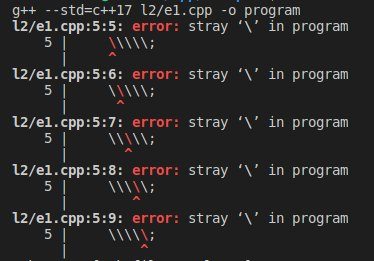
\includegraphics[width=1\textwidth]{l2img1.png}
    \caption{Пример лексической ошибки.}
    \label{l2img1}
\end{figure}

Здесь stray можно перевести как "заблудший" или "заплутавший". Компилятор не смог это как-то интерпетировать.

Приведем более подробные примеры синтаксических ошибок.

\begin{minted}{cpp}
#include <iostream>

int main() {
    int x
    std::cin >> x;
    std::cout << x + 5;
}
\end{minted}

\begin{figure}[h]
    \centering
    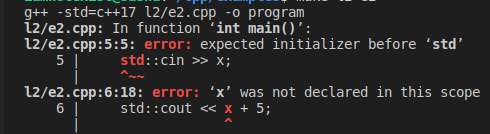
\includegraphics[width=1\textwidth]{l2img2.png}
    \caption{Пример синтаксической ошибки 1.}
    \label{l2img2}
\end{figure}

На рисунке \ref{l2img2} написано, что компилятор ожидал инициализацию перед std.
Иначе говоря он парсит строки 5 и 6 как одно выражение, так как в строке пять нет ';',
однако после объявления переменной компилятор ожидает либо ничего, либо ее инициализацию,
а так как дальнейшее инициализацией никак не является, то это ошибка. Так как эта ошибка возникла из-за  отсуствия ';' 
и была обнаружена на этапе синтаксического разбора она считается синтаксической.

Далее компиляция не прервалась и было обнаружено, что переменная \underline{x} не была объявлена, поскольку предыдущее выражение ошибочно.
Стоит отметить, что компилятор не сказал об использовании необъявленной переменной в 5-ой строке после \underline{std::cin}, так как уже отловил в этом выражении синтаксическую ошибку.
Выражения не всегда рассматриваются на предмет ошибок до конца, да и здесь это не требуется.

\begin{minted}{cpp}
#include <iostream>

int main() {
    int x;
    std::cin >> x;
    std::cout << x + 5;
    x + 5 + ;
}
\end{minted}

\begin{figure}[h]
    \centering
    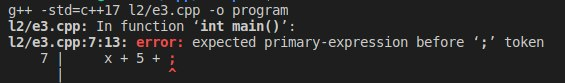
\includegraphics[width=1.3\textwidth]{l2img3.png}
    \caption{Пример синтаксической ошибки 2.}
    \label{l2img3}
\end{figure}

Поскольку '+' здесь используется как бинарный оператор, а после стоит ';', то перед ';' ожидается
некое \underline{primary-expression}, о котором будет рассказано позже.

Компилятор старается не завершать компеляцию, чтобы выдать как можно больше ошибок сразу, однако у него не всегда это получается.
Ошибки, при которых компиляция останавливается, называются \textbf{фатальными}.

\begin{minted}{cpp}
#include <iostream>
#include <aaaaaaaa>

int main() {

}
\end{minted}

\begin{figure}[h]
    \centering
    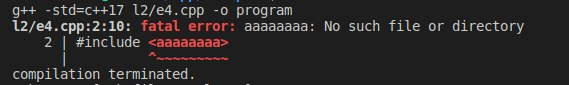
\includegraphics[width=1.3\textwidth]{l2img4.png}
    \caption{Пример синтаксической ошибки 3. Фатальная ошибка.}
    \label{l2img4}
\end{figure}

Примером фатальной ошибки будет являться подключение файла, которого не существует.

Можно привести такой неформальный пример синтаксической ошибки
\begin{center}
Я пошел лес грибы.
\end{center}
Вроде и все понятно, но синтаксически неверно.

А вот какой пример можно привести для семантической ошибки
\begin{center}
Я ем стол.
\end{center}
С точки зрения синтаксиса здесь все верно, однако есть стол это как-то странно.
Иначе говоря мы понимаем, какую пищу может есть человек, а какую нет. Человек не может есть стол.
Подобная ошибка называется семантической.

Другими словами если мы пытаемся совершить что-то невозможное, то это \textbf{семантическая ошибка}.

\begin{minted}{cpp}
#include <iostream>

int main() {
    int x;
    std::cin >> x;
    std::cout << x.size();
}
\end{minted}

\begin{figure}[h]
    \centering
    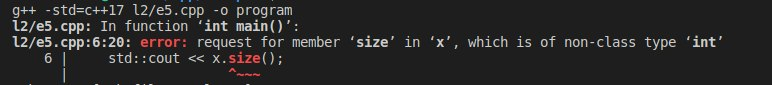
\includegraphics[width=1.3\textwidth]{l2img5.png}
    \caption{Пример семантической ошибки 1.}
    \label{l2img5}
\end{figure}

Мы пытаемся применить метод \underline{.size()} к переменной целочисленного типа,
однако это невозможно, поскольку переменная целочисленного типа не обладает методом \underline{.size()}.
О методах мы узнаем позже.

\begin{minted}{cpp}
int main() {
    int x;
    int a;
    int b;
    x++ = a + b;
}
\end{minted}

\begin{figure}[h]
    \centering
    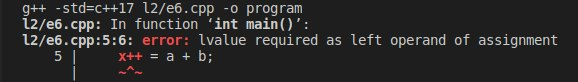
\includegraphics[width=1.3\textwidth]{l2img6.png}
    \caption{Пример семантической ошибки 2.}
    \label{l2img6}
\end{figure}

Это тоже семантическая ошибка, поскольку тому, что стоит слева от '='
невозможно присвоить что-либо, так как то что слева не является \underline{lvalue}.
О том что такое \underline{lvalue} мы тоже поговорим позднее.

Заметим, что на рисунке \ref{l2img2} также показана семантическая ошибка, так как мы пытаемся использовать необъявленную переменную.
\begin{minted}{cpp}
int main() {
    int x;
    int x;
}
\end{minted}

\begin{figure}[h]
    \centering
    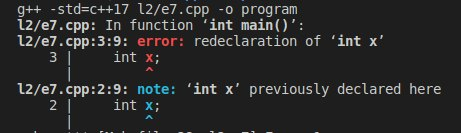
\includegraphics[width=1.3\textwidth]{l2img7.png}
    \caption{Пример семантической ошибки 3.}
    \label{l2img7}
\end{figure}

Вспомним о повторном объявлении переменной. Это тоже семантическая ошибка, рисунок \ref{l2img7}.

Также иногда семантическая ошибка возникает при неоднозначном обращении, рисунок \ref{l2img8}.

\begin{minted}{cpp}
#include <iostream>

namespace N {
    int x;
}

using namespace N;

int x = 0;

int main() {
    std::cin >> x;
    std::cout << x + 5;
}
\end{minted}

\begin{figure}[h]
    \centering
    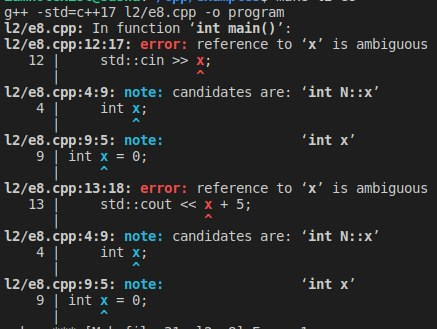
\includegraphics[width=1\textwidth]{l2img8.png}
    \caption{Пример семантической ошибки 4.}
    \label{l2img8}
\end{figure}

Здесь переменная 'x' объявлена в \underline{пространстве имен} 'N', а далее, строкой

\begin{minted}{cpp}
using namespace N;
\end{minted}

сливается с глобальной областью видимости.

Так как переменные объявлены в разных областях видимости здесь нет ошибки повторного объявления,
значит это две разные переменные. Однако после сливания не понятно, к какой именно переменной идет обращение.


Помимо ошибок компиляции существуют ошибки, которые возникают во время исполнения программы.
Они называются \textbf{Runtime error} (\textbf{RE}).

Примеры ошибок времени выполнения:

\begin{enumerate}
    \item Слишком далекий выход за границу массива
    \item Бесконечная рекурсия
    \item Целочисленное деление на ноль
\end{enumerate}

Первые и вторые примеры это примеры одной ошибки, которая называется \textbf{Segmentation fault}.
При этой ошибке программа обращается к памяти, которая ей не принадлежит.


\begin{minted}{cpp}
#include <iostream>

int main() {
    int a[100];

    a[10000000] = 1;
}
\end{minted}

\begin{figure}[h]
    \centering
    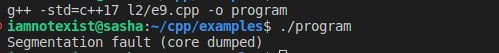
\includegraphics[width=1\textwidth]{l2img9.png}
    \caption{Segmentation fault.}
    \label{l2img9}
\end{figure}

При попытке исполнения этой программы получим результат Segmentation fault.
Так как программа работает с памятью, которую ей выдала операционная система, работа с не ее памятью может привести к прекращению работы.
Таким образом борется с тем что мы пытаемся работать не со своей памятью.


Аналогичный результат будет и при бесконечной \underline{рекурсии}:
\begin{minted}{cpp}
void f() {
    f();
}

int main() {
    f();
}
\end{minted}
Здесь Segmentation fault происходит потому, что при вызове \underline{функции} программе необходимо запомнить \underline{адрес возврата}.
Поскольку вызовы не будут прекращаться, программа прывысит лимит выделенной памяти и попытается записать информацию в память, которая ей не принадлежит.
Так как адреса возврата запоминаются на \underline{стеке}, то это приводит к его переполнению~--- \textbf{Stack overflow}.

Третий же пример ошибки выполнения под названием \textbf{Floating point exception}.

\begin{minted}{cpp}
#include <iostream>

int x;

int main() {
    std::cin >> x;
    std::cout << x / 0;
}
\end{minted}

\begin{figure}[h]
    \centering
    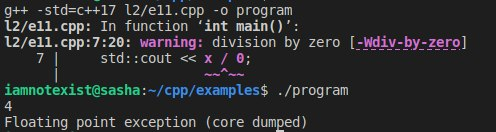
\includegraphics[width=1\textwidth]{l2img10.png}
    \caption{Floating point execption.}
    \label{l2img10}
\end{figure}

При компиляции компилятор выдал предупреждение \textbf{Warning}, информацию о том, что в коде возможно что-то не так.
При попытке запуска и после ввода значения программа падает с ошибкой Floating point excception.

По другому падение программы при подобных ошибках называют \textbf{аварийным завершением программы}.
Также примером RE бывает \textbf{Illegal instruction}. Это происходит когда машинный код поврежден и процессор не может его выполнить.

Помимо этого в C++ есть и другие варианты ошибок. Поговорим про \textbf{Undefined behavior}, что переводится как неопределенное поведение.
Неопределенное поведение это когда при некоторой ситуации в коде программы компилятор перестает гарантировать что либо относительно поведения такого кода.

Приведем абстрактный пример.
Пусть есть олимпиадная задача по информатике, в который подробно описаны входные данные.
Решением будет программа, которая обработает входные данные исходя из ограничений и выдаст ответ.
Но что она будет делать если ей гарантировали, к примеру, неотрицательные числа во входных данных, а дают отрицательные?
По сути программа может делать все что угодно.

Так и с компилятором. У компилятора есть входные данные~--- код на C++, которые ограничены его стандартом. И в самом стандарте прописаны некоторые оговорки о том, что
при каких-то действиях будет возникать UB.

При наличии в коде инструкций, которые классифицируются как UB, компилятор может делать все что угодно. Существует даже шутка о том, что компилятор может поджечь монитор.
Тем самым при наличии в коде UB код является некорректными данными для компилятора.

Примеры неопределенного поведения:

\begin{enumerate}
    \item Выход за границу массива.
    \item Переполнение переменной типа \underline{int}.
\end{enumerate}

При выходе за границу массива возможен RE, но он также может и не произойти.
При этом RE будет следствием UB.

Приведем пример UB при переполнении \underline{int}.

\begin{minted}{cpp}
#include <iostream>
int main() {
    for (int i = 0; i < 300; i++)
        std::cout << i << " " << i * 12345678 << std::endl;
}
\end{minted}

Здесь будет выводится 'i' и 'i умноженное на 12345678', после будет перевод строки.
Все это будет происходить в цикле.
Попробуем скомпилировать и запустить.

\begin{figure}[h]
    \centering
    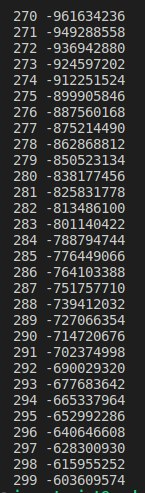
\includegraphics[width=0.2\textwidth]{l2img11.png}
    \caption{Вывод примера 12.}
    \label{l2img11}
\end{figure}

На выходе получаем рисунок \ref{l2img11}.

В начале вывода числа будут нормальными, но в потом они будут отрицательными.
На 174 шаге int переполнился.

Поробуем скомпилиривать код с параметром оптимизации \textbf{-O2}.
Параметр оптимизации говорит компилятору о том, что если код можно преобразовать в тождественно такой же код, 
но более простой, то он это делает. В зависимости от параметра он может делать это по-разному.

Бывают следущие параметры
\begin{itemize}
    \item -O0. При этом параметры оптимизации не производятся.
    \item -O1. Простые оптимизации.
    \item -O2. Более мощные оптимизации.
    \item -O3. Максимальные оптимизации.
\end{itemize}

При флаге -O2 код будет работать быстрее.

\begin{figure}[h]
    \centering
    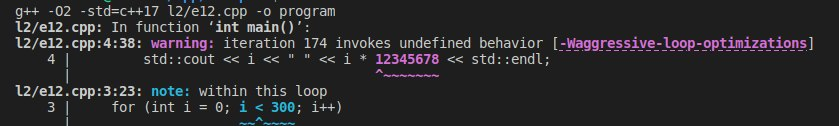
\includegraphics[width=1.3\textwidth]{l2img12.png}
    \caption{Вывод примера 12 при компиляции с флагом -O2.}
    \label{l2img12}
\end{figure}

Компилятор заметил, что на 174 итерации цикла происходит UB.
При попытке запуска программы она входит в вечный цикл или \textbf{зацикливается}.

После оптимизации компилятором цикл, который шел 300 итераций, вдруг зациклился.
Компилятор увидел UB из-за aggressive-loop-optimization. Это случилось потому, что компилятор заметил, что 'i' 
умножается на '12345678'. В предположении того, что код корректен, 'i' не может превзойти 173, так как в предположении корректности \underline{int} не переполняется.
Значит \underline{условие в цикле 'i < 300'} никогда не будет ложным, а значит, для избежания лишних сравнений компилятор может подставить туда истину.
Поэтому программа и зацикливается.

UB~--- самое плохое, что может быть в коде. Дело в том, что например ошибки компиляции идут во благо. То, к чему компилятор придирается, дает возможность избежать ошибок в run-time.
Если компилятор чего-то не нашел, значит может произойти что-то плохое в run-time, что будет сложно отловить. Существуют даже специальные слова, которые не влияют на код,
но без них компиляция не будет происходить.

Почему тогда компилятор не отлавливает RE во время компиляции? Просто потому что это может быть невозможно с точки зрения математики.
У этого даже существует название~--- \textbf{проблема остановки}. Иначе говоря, глядя на программу, невозможно всегда сказать, произойдет ли какое-то действие или нет.

Почему UB нельзя классифицировать как RE и аварийно завершать программу? Например в Jave так и происходит, однако C++ не про это.
С++ нацелен на производительность и эффективность.

Абстрактный пример: 
\begin{center}
Если мама постоянно будет проверять, надели ли мы шапку, перед тем как пойти на улицу, это в скором времени начнет нас бесить.
\end{center}

Проверки в run-time требуют определенного времени, а мы не хотим терять в производительности.
За счет существования UB C++ выигрывает в эффективности.

Помимо UB в C++ существует неспецифицированное поведение
\textbf{Unspecified behavior (UC)}.
Иначе говоря, в некоторых ситуациях у компилятора есть ограниченная свобода действий.
Однако результат должен быть в каких-то рамках.

\begin{minted}{cpp}
#include <iostream>

int f() {
    std::cout << 1;
    return 0;
}

int g() {
    std::cout << 2;
    return 0;
}

int main() {
    f() + g();
}
\end{minted}

Вывод этой программы будет неспецифицированным.
Мы не можем с уверенностью сказать, что выведет эта программа.
По стандарту она может выводить как 12 так и 21. Это связано с тем,
что компилятор может запускать функции в данном случае в любом порядке.

Поробуем скомпилировать и запустить эту программу.

\begin{figure}[h]
    \centering
    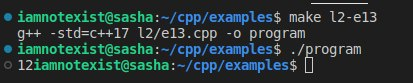
\includegraphics[width=0.5\textwidth]{l2img13.png}
    \caption{Пример неспецифицированного поведения, g++.}
    \label{l2img13}
\end{figure}

В данном случае программа вывела 1 потом 2.

Попробуем скомпилировать другим компилятором и запустить.

\begin{figure}[h]
    \centering
    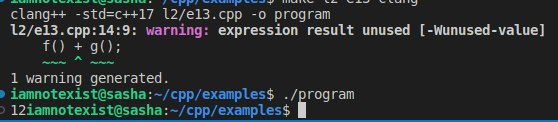
\includegraphics[width=0.8\textwidth]{l2img14.png}
    \caption{Пример неспецифицированного поведения, clang++.}
    \label{l2img14}
\end{figure}

Вывод программы остался тем же, однако заметим разницу в компиляторах.
clang++ дал информацию о том, что мы не используем результат вычисления функций, выдавая Warning.

В стандарте нет требования о том, что при вычислении выражения 'a + b' компилятор должен вычислить сначала 'a' и только потом 'b'.
Поэтому код вызывает неспецифицированное поведение.

Однако это не стоит путать с порядком вычисления самого выражения.


\begin{minted}{cpp}
#include <iostream>

int f() {
    std::cout << 1;
    return 2;
}

int g() {
    std::cout << 2;
    return 3;
}

int main() {
    std::cout << f() + g() * g();
}
\end{minted}


Результат выражения однозначно определяется и равен 11,
однако результат выражения не связан с порядком вычисления f() и g().
f() и g() могли вычисляться в любом порядке, это не определено.

\begin{minted}{cpp}
f(g(), h());
\end{minted}

Выше также пример неспецифицированного поведения, g() и h() могут вычисляться в любом порядке.

Не все в стандарте специфицированно точно, потому что это не так важно, а некоторым компиляторам проще делать это по-своему.

Хочется добавить, что существуют некоторые полезные флаги компиляции.

Если посмотреть на рисунки \ref{l2img13} и \ref{l2img14}, можно заметить, что clang++ отловил warning, а g++ нет.
Если добавил флаг \textbf{-Wall}, то компилятор будет искать warning тчательнее. Флаг \textbf{-Wextra} это усилит.

\begin{figure}[h]
    \centering
    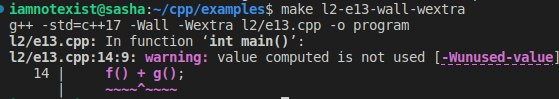
\includegraphics[width=0.8\textwidth]{l2img15.png}
    \caption{Компиляция g++ с -Wall и -Wextra.}
    \label{l2img15}
\end{figure}

По умолчанию warning не припятствуют компиляции, однако если написать флаг \textbf{-Werror}, каждый warning превратится в error, что не даст некорректной программе скомпилироваться.

\begin{figure}[h]
    \centering
    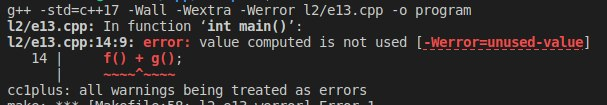
\includegraphics[width=0.8\textwidth]{l2img16.png}
    \caption{Компиляция g++ с -Werror.}
    \label{l2img16}
\end{figure}

Благодаря этому мы сможем по максимуму избежать UB.

\subsection{Declarations, definitions and scopes.}

На самом деле наши предыдущие коды это последовательные объявления некоторых сущностей одной за другой,
которые кончались main().

Формально сама программа это последовательность объявлений, с точки зрения компилятора.

Можно объявлять (вводить в рассмотрение) разные сущности.
Например, переменные:

\begin{center}
type id [= init];
\end{center}

Тип переменной, ее имя (идентификатор).
Так же как необязательная часть возможна ее инициализация.

Также можно объявлять функции.

\begin{center}
type fid(type1 id1, ..., typeN idN);
\end{center}

Тип функции, ее имя (идентификатор), типы и идентификаторы аргументов в круглых скобках через запятую.

Можно объявлять свои собственные типы.

\begin{center}
struct S; \\
class C; \\
union U;
\end{center}

Можно объявлять пространства имен.

\begin{center}
namespace N \{\}
\end{center}

Можно объявлять \textbf{alias}~--- другие названия чего-то объявленного (псевдонимы).

\begin{center}
typedef shortname longTypeName; \\
using shortname = longTypeName;
\end{center}

Компилятор будет транслировать shortname как longTypeName, что может сократить код.

Таким образом объявления \textbf{declarations} дают знать компилятору о каких-то сущностях.
\textbf{Definitions}~--- определения сущностей.

\begin{minted}{cpp}
int main() {
    int x;
}
\end{minted}

В этом коде была объвлена переменная 'x'. Однако по стандарту она сразу же и определяется, в данном случае каким-то рандомным значением, которое лежало на стеке.

\begin{minted}{cpp}
int main() {
    int x = 5;
}
\end{minted}

Здесь мы сами определяем переменную 'x' и даем ей значение 5.

С функциями все немного по-другому.

\begin{minted}{cpp}
int g() {
    f();
}

int f() {
    g();
}

int main() {

}
\end{minted}

В этом коде хочется использовать фунцию f() в определении функции g(), 
а функцию f() использовать в определении функции g(). Такой код не скомпилируется потому что на момент определения g() функция f() не объявлена.

\begin{minted}{cpp}
int f();

int g() {
    f();
}

int f() {
    g();
}

int main() {

}
\end{minted}

Здесь мы заранее объявили функцию f() поэтому код скомпилируется.

Таким образом для функции можно дать определении позже, но если мы хотим ее использовать, оно должно быть.

Существует некоторое правило: \textbf{One definition rule.}

Оно гласит в частности, что каждая функция и каждая переменная должна быть ровно один раз определена, если она не определена один раз, то ей нельзя пользоваться.
Объявлять функцию можно сколько угодно раз.

\begin{minted}{cpp}
int f();

int f();

int g() {
    f();
}

int f() {
    g();
}

int main() {

}
\end{minted}

Поэтому такой код скомпилируется. Поскольку переменная единвроменно определяется при создании такой трюк c ними уже не пройдет.